% University of Glasgow School of Computing Science project template
% Dissertation outline for MSc project planning.
\documentclass{l4proj}

\usepackage{pdfpages}
\usepackage{xeCJK}
% Prefer Noto CJK when it is installed locally. Overleaf's XeLaTeX setup can
% fall back to the Fandol fonts distributed with TeX Live.
\IfFontExistsTF{Noto Serif CJK SC}{
  \setCJKmainfont{Noto Serif CJK SC}
  \setCJKsansfont{Noto Sans CJK SC}
  \setCJKmonofont{Noto Sans Mono CJK SC}
}{
  \setCJKmainfont{FandolSong-Regular.otf}
  \setCJKsansfont{FandolHei-Regular.otf}
  \setCJKmonofont{FandolFang-Regular.otf}
}

% Keep the Glasgow template's page geometry and fonts while matching the
% reference dissertation's compact contents and centred chapter openers.
\setcounter{tocdepth}{2}
\renewcommand{\cftdot}{.}
\renewcommand{\cftbeforechapskip}{3pt}
\renewcommand{\cftchapafterpnum}{\vskip 1pt}
\titleformat{\chapter}[display]
  {\normalfont\Huge\bfseries\sffamily\filcenter}
  {}{0pt}{}
\titleformat{name=\chapter,numberless}[display]
  {\normalfont\Huge\bfseries\sffamily\filcenter}
  {}{0pt}{}
\titlespacing*{\chapter}{0pt}{0pt}{36pt}
\lstset{breaklines=true,breakatwhitespace=false}

\begin{document}

\renewcommand{\abstractname}{摘要}
\renewcommand{\contentsname}{目录}
\renewcommand{\figurename}{图}
\renewcommand{\tablename}{表}
\renewcommand{\bibname}{参考文献}
\renewcommand{\appendixname}{附录}
\renewcommand{\appendixtocname}{附录}

%==============================================================================
%% METADATA
\title{二维机器人抓取检测的受控比较：传统视觉、VLM 引导几何与 CNN 后端}
\author{Pang Zhenkun}
\date{MSc Robotics \& Artificial Intelligence\\Supervisor: Dr Jan Paul Siebert\\2026}

\maketitle

%==============================================================================
%% ABSTRACT
\begin{abstract}
机器人抓取检测需要同时确定目标位置和夹爪几何，但传统整图分割易受背景干扰，开放词汇定位能否为轻量抓取后端提供可靠输入仍缺少受控证据。本研究使用 Cornell Grasping Dataset 的 885 幅 RGB 图像，比较传统计算机视觉、Grounding DINO 加几何后端、单头 CNN 与多头 CNN。修正后的 Cornell 指标要求同一个正标注同时满足 IoU 与角度门槛。加入开放词汇定位后，几何流程成功率由 58.98\%（522/885）提高至 74.46\%（659/885），配对精确 McNemar 检验 $p=5.24\times10^{-33}$。共同 image-wise 五折下，多头 CNN 为 75.82\%（671/885），单头为 74.69\%（661/885）；差异仅 1.13 个百分点且 $p=0.373$，不支持显著架构优势。CNN 的平均最佳 IoU 较高，几何后端的条件角度误差较低，说明模型选择不能只看单一成功率。结论限于 RGB-only、image-wise、小型单物体数据和离线矩形评价。补充 PyBullet 仿真完成了真值控制链与感知执行 pilot：两个斜视运行均有约 25--27\,mm XY 偏差并抬升失败；历史顶视运行同时把抓取深度由 $+5$\,mm 改为 $-25$\,mm，偏差降至 0.76\,mm 并抬升成功。因此它只证明固定场景中“顶视 + 深抓取”联合配置的可行性，尚不能把差异单独归因于相机，也不构成仿真成功率。
\end{abstract}

%==============================================================================
%% ACKNOWLEDGEMENTS
\chapter*{致谢}
感谢导师 Dr Jan Paul Siebert 在研究设计、实验解释和论文写作方面提供的指导与反馈。感谢 University of Glasgow School of Computing Science 提供完成本项目所需的学习与研究环境。

%==============================================================================
%% EDUCATION REUSE CONSENT FORM
% Uncomment and complete these lines only if you consent to educational reuse.
%\def\consentname {Pang Zhenkun}
%\def\consentdate {Date}
\educationalconsent

%==============================================================================
\tableofcontents

%==============================================================================
\chapter{引言}
\pagenumbering{arabic}

\section{背景与研究动机}
机器人要在未知环境中操作物体，首先必须从视觉观测中确定“抓哪里”和“以什么方向抓”。二维抓取检测把这一问题表示为图像平面上的有向矩形，为比较不同感知方法提供了可计算接口。然而，传统整图分割容易受到背景、阴影和反光影响；监督学习模型则依赖抓取标注与训练分布。开放词汇视觉语言模型能够根据文本定位目标，为抓取系统提供另一种前端，但目标检测框描述的是物体范围，而不是可夹持部位，两者之间仍需要可靠的几何或学习后端。

已有研究常同时改变 RGB/RGB-D 输入、网络结构、数据划分和输出形式，因而很难判断性能变化究竟来自目标定位、抓取回归还是实验协议。本研究选择模块化设计：以传统整图计算机视觉为参照，加入 Grounding DINO 定位前端后分别连接确定性几何后端、单头 CNN 和多头 CNN。共同裁剪使后端比较保持输入一致，确定性重复实验和共同 fold manifest 则使统计口径可审计。研究动机不是追逐单一最高准确率，而是识别各模块实际解决了什么问题、仍会在哪里失败。

\section{研究问题}
本论文围绕三个递进问题展开：

\begin{enumerate}
    \item 在 Cornell RGB 单目标图像和通用文本提示条件下，Grounding DINO 是否能改善传统整图几何流程？
    \item 当几何、单头 CNN 与多头 CNN 接收共同 VLM crop 时，各后端在空间重合、方向估计和失败类型上有何优势与局限？
    \item 在字节相同的 image-wise 五折 manifest 下，多头 CNN 是否优于单头 CNN，其增益是否在不同指标和 fold 上一致？
\end{enumerate}

第一个问题隔离定位前端的作用，第二个问题研究手工先验与数据驱动回归的差异，第三个问题进一步控制训练样本划分，只检验输出头组织方式。三者共同回答开放词汇定位如何以可解释、可复现的方式嵌入二维抓取管线。

\section{研究意义}
学术上，本研究通过共享定位裁剪减少模块混杂，补充 VLM 前端与轻量抓取后端之间的受控证据。工程上，定位器和后端可以独立替换，便于在算力有限的平台上诊断误差来源。更重要的是，论文同时报告均值、波动和逐样本互补性，使结论强度与现有证据相匹配。

\section{论文结构}
第二章按技术主题批判性回顾抓取矩形、深度学习、开放词汇定位和语言驱动抓取，并提出研究缺口。第三章界定项目目标、交付物、系统边界和成功判据。第四章说明模块化系统设计及四类感知后端的实现。第五章给出 Cornell 与 PyBullet 的实验框架、评价协议、统计方法和研究伦理。第六章按三个研究问题报告 Cornell 定量与定性结果，并另列补充仿真结果。第七章综合解释主要发现、文献联系、失败来源与证据局限。第八章逐条回答研究问题，总结贡献并提出未来工作。附录记录复现命令、环境、结果产物与固定划分的历史用途。

%==============================================================================
\chapter{背景与文献综述}

\section{机器人抓取检测}
机器人抓取检测处于视觉感知与操作执行之间：系统不仅要回答“物体在哪里”，还要给出夹爪中心、开口尺度和接近方向等几何量。目标检测框只描述物体所占区域，抓取则受到表面形状、遮挡、夹爪宽度和碰撞风险约束，因此语义上正确的目标框并不自动构成可执行抓取。实际机器人还需要深度恢复、运动规划、控制与接触反馈；二维图像实验只能评价感知阶段，不能把离线矩形匹配直接称为物理抓取成功。

早期方法常把物体分割、轮廓提取和主轴分析组合成确定性流程。这类方法计算成本低，能把预测原因追溯到阈值、连通区域或几何矩；在背景简单、物体与桌面对比明显时具有工程吸引力。然而，颜色阈值和最大轮廓隐含了“单物体、背景稳定、轮廓完整”等强假设，光照、阴影、反光或定位框过松都可能改变主轴。它们表达了明确的几何先验，却很难从数据中学习不同物体的可抓取区域。

Jiang 等人把平行夹爪抓取表示为图像平面上的有向矩形，以两条平行边对应夹爪接触板，使抓取检测可以使用视觉检测和学习方法评价\citep{jiang2011efficient}。这一抽象把复杂六自由度操作压缩为中心、宽度、高度与角度，适合桌面单物体研究，也成为 Cornell 基准的核心表示。其优势是标注和比较方便；不足是忽略接近深度、表面法向、碰撞和夹持力，同一物体还可能对应多个同样有效的矩形。因此，单个预测与某个标注不重合，未必意味着抓取在物理上不可行；反过来，矩形匹配成功也不保证机器人能够完成动作。

\section{二维抓取矩形与 Cornell 基准}
Cornell Grasping Dataset 为每幅 RGB-D 图像提供多个正抓取矩形，推动了二维抓取方法的统一比较。常用 rectangle metric 要求预测矩形与任一正标注的交并比（intersection over union, IoU）大于 0.25，同时平行夹爪的方向误差小于 $30^\circ$。该规则同时约束空间重合与方向，但阈值二值化会隐藏接近边界的差异：IoU 为 0.249 与 0.251 的预测几何质量非常接近，最终标签却相反。因此，成功率应与平均 IoU、角度误差及案例分析一起报告。

Lenz 等人用 RGB-D 输入学习候选抓取的特征和分数，并以小网络进行第一阶段筛选、较大网络重新评价少量候选\citep{lenz2015deep}。两阶段设计减少近穷举搜索的计算量，结构化正则也利用了颜色、深度和表面法向等多模态信息。它的重要贡献不仅是提高矩形指标，还在 Baxter 与 PR2 上进行了执行实验，显示感知输出能够嵌入完整机器人流程。不过，其候选搜索、RGB-D 特征和机器人实验与本项目的 RGB 裁剪单矩形回归不同；物理执行率也不能与 Cornell 离线成功率直接排列比较。

Redmon 与 Angelova 将候选搜索改为卷积神经网络（convolutional neural network, CNN）直接回归，并进一步用网格输出多个抓取，展示了全局单次前向预测的实时性\citep{redmon2015real}。相较 Lenz 的逐候选评分，它减少了推理步骤并把特征提取和矩形估计联合优化；但全局回归会把多个有效抓取压缩为一个目标，且其已报告结果使用 RGB-D 与标准五折。它支持“图像到矩形”的技术路线，却不能证明不同输入模态或不同 fold 成员下的数字直接可比。

Cornell 常见 image-wise 与 object-wise 两种划分。Image-wise 将图像分配到折中，同一物体的相邻视角可能同时进入训练与测试；object-wise 则把物体实例隔离，更接近未见物体泛化，通常也更难。Lenz 的结果表明确同时报告这两种设置，并指出 object-wise 更容易暴露过拟合。若没有权威的图像到物体实例映射，仅按下载目录编号分组不能重建 object-wise。本项目因此只把可审计的 image-wise 五折称为图像级交叉验证，不声称已经测试未见物体。Cornell 规模较小、场景多为单物体和简洁背景，也不足以代表开放世界杂乱场景。

评价协议的透明度还影响复现。不同研究可能采用不同图像缩放、角度规范化、增强方式和“与任一真值匹配”的实现；即使都写作 image-wise 五折，fold 成员也未必相同。若只给平均成功率而不保存样本清单，后续研究无法判断差异来自模型还是划分。本项目因此保存 manifest、随机种子和哈希，并在相同样本上计算 pooled 指标。Pooled 结果回答全部测试预测合并后的总体表现，fold 标准差则反映划分间波动，两者含义不同，不能互相替代。

\section{传统计算机视觉与深度学习方法}
传统计算机视觉基线通常在整图上进行颜色或亮度分割，再从最大轮廓计算中心、包围框与主轴角度。其优点是无需训练、行为可解释，并可快速诊断“分割错”还是“几何估计错”；缺点是阈值对采集条件敏感，而且最大连通区域不一定是目标。对本项目而言，这类基线仍有价值，因为它建立了不使用语义定位时的参照，使 Grounding DINO 带来的变化能够与后端学习效果分开。

深度学习逐步减少了手工特征。Kumra 与 Kanan 使用深层残差网络处理 RGB-D 并进行抓取分类和回归\citep{kumra2017robotic}，说明更强视觉表征能够改善候选判断，但模型容量、深度通道和增强策略同时发生变化，难以把提升归因于某一个因素。学习方法还依赖训练分布；小数据集上的较大网络可能记忆物体外观，因此随机种子、验证集选择和测试隔离都应写清楚。

Morrison 等人的生成式抓取卷积神经网络（Generative Grasping Convolutional Neural Network, GG-CNN）从单幅深度图在每个像素预测抓取质量、角度和宽度\citep{morrison2018closing}。密集输出绕开离散候选采样，能表达多个位置，并可在闭环控制中快速更新。其用 $\sin(2\theta)$ 和 $\cos(2\theta)$ 表示平行夹爪的 $\pi$ 周期方向，避免 $-\pi/2$ 与 $\pi/2$ 边界处的回归不连续，这一表示直接启发本项目的方向头。限制在于 GG-CNN 依赖深度，并将空间预测保留为图，因此与 RGB 裁剪后的单矩形输出仅为有限可比；其动态机器人结果更不能作为本项目离线指标的基线。

后续 GR-ConvNet 以生成式残差网络同时预测质量、角度和宽度图\citep{kumra2020antipodal}，Gaussian-guided 方法进一步以高斯形式塑造抓取质量监督\citep{li2022gaussian}。这些方法的共同方向是密集多抓取，而非单个全局参数：它们保留局部候选，适合从多个可行解中选择。与此同时，它们常使用 RGB-D、较强增强和不同训练协议。论文中更高的 Cornell 百分比反映了领域进展，却不能脱离输入模态、数据划分、输出形式与评价实现组成公平排行榜。本项目采用轻量单矩形 CNN，目的不是声称达到最新水平，而是在共同定位裁剪下进行受控后端比较。

\section{视觉语言模型与开放词汇定位}
视觉语言模型（vision-language model, VLM）通过联合视觉和文本表示，使自然语言能够参与目标选择。CLIP 以大规模图文对学习可迁移的对齐空间，表明自然语言监督可以支持零样本视觉识别\citep{radford2021learning}。然而，图像级相似度不能给出目标的精确空间范围，也不包含夹爪几何，因此仍需定位模型和抓取后端。

Grounding DINO 将 Transformer 检测器与 grounded pre-training 结合，使用类别名或指代表达进行开放集目标检测\citep{liu2023grounding}。其语言引导查询选择与跨模态解码能够在没有 Cornell 专项训练的情况下根据提示返回目标框。对单目标 Cornell 图像，这提供了一种通用前端：先把目标从背景中裁出，再用几何规则或 CNN 估计抓取。该模块的优势是把语义定位与抓取回归解耦，后端可以替换；主要风险是 prompt、置信度阈值和框边界会改变裁剪内容。每幅图都返回框的 885/885 定位覆盖率只说明接口没有空输出，并不等于框准确，也不等于抓取可行。

Vuong 等人更直接研究语言驱动抓取，在 Grasp-Anything++ 上把自然语言指定的目标抓取作为条件生成问题，并使用扩散模型预测抓取\citep{vuong2024language}。它显示语言不仅可选类别，还可描述杂乱场景中的目标或部位，研究范围比“通用 prompt 定位单个 Cornell 物体”更广。其大规模数据、语言指令、生成式输出及真实机器人展示是重要优势；但数据集和指标均不同，本项目不能把其结果当作 Cornell 数值基线。两者的联系是语言条件可以承担目标选择，区别是本项目刻意固定通用提示，只检验开放词汇定位框能否为传统几何或轻量回归提供更好的输入。

\section{轻量与参数高效适配}
参数高效微调为大模型域适配提供另一条路线。低秩适配（Low-Rank Adaptation, LoRA）冻结原模型权重，只学习低秩增量\citep{hu2021lora}；量化低秩适配（Quantized LoRA, QLoRA）进一步结合低比特量化，降低训练显存\citep{dettmers2023qlora}。这些方法说明无需更新全部参数也可调整大型模型，但其原始研究重点并非二维抓取，实际收益仍需任务数据和独立实验验证。

本研究没有对 Grounding DINO 实施 LoRA 或 QLoRA。原因不是否认适配价值，而是核心问题要求先建立清晰控制变量：若同时改变定位器权重、提示和抓取后端，性能变化将无法归因。GTX 1650 Ti 的 4\,GB 显存也限制了大模型训练范围。因此，预训练 VLM 保持冻结，只有轻量 CNN 后端在 Cornell 标注上训练；参数高效适配被保留为后续研究，而非未经验证写入当前贡献。

\section{研究缺口}
既有研究分别推进了矩形表示、RGB-D 深度回归、密集抓取生成与语言驱动选择，但仍缺少一种面向本项目条件的受控证据：在 RGB-only、单目标 Cornell 和不提供样本类别的通用 prompt 下，开放词汇定位究竟贡献了多少；当定位裁剪完全相同时，确定性几何、单头 CNN 与多头 CNN 的差异又来自哪里。现有高性能论文多改变了输入模态、数据划分或输出形式，无法直接回答这个模块归因问题。

本论文据此构建三条相互关联的流程。首先，以整图传统视觉作为不含语义定位的基线；其次，把共同 Grounding DINO crop 交给几何后端；最后，在字节相同的 crop 上训练单头与多头轻量 CNN。固定目录结果用于与早期开发产物配对，五个随机种子检验训练随机性，共同 image-wise 五折 manifest 检验图像划分变化。研究目的不是宣布新的 Cornell 最新水平，而是通过可复现的模块化比较，回答定位前端、学习后端和多任务分头各自的作用，并明确 image-wise、object-wise、离线矩形与物理抓取之间的证据边界。

这一缺口也决定了论文的批判立场：若定位前端带来最大变化，则应优先研究裁剪质量而非盲目扩大后端；若几何与 CNN 在不同误差维度互补，则单一成功率会掩盖设计机会；若多头只产生有限增益，则结果应按效应大小和折间稳定性解释，而不能仅凭均值上升作强结论。由此，文献综述不只提供方法清单，也给出了后续研究问题、控制变量和结论强度的依据。

%==============================================================================
\chapter{项目描述与目标}

\section{项目概述}
本项目面向开放词汇定位辅助的二维机器人抓取检测，目标是在统一数据、输入模态与评价实现下，分离定位前端、确定性几何后端和轻量学习后端各自带来的影响。项目以 Cornell RGB 图像上的离线矩形评价为主线，并以固定 PyBullet 场景补充检查从二维感知到三维坐标和物理执行的数据流。该组织把“系统要实现什么”“如何实现”与“如何实验验证”分开，使后续章节能够逐层对应研究问题和证据。

\section{系统边界与模块化数据流}
三个主要研究问题仍限定于 Cornell 数据集上的离线二维 RGB 感知，不在这些性能比较中融合深度。论文另以固定 PyBullet 场景进行补充仿真验证，分为三层：(1) 检验九个二维抓取中心能否通过米制深度和相机矩阵恢复为目标表面世界点；(2) 以真值姿态验证分阶段运动--接近--闭合--抬升控制链，再加载由感知生成的计划执行完整链条；(3) 记录斜视失败与历史顶视成功的联合干预 pilot。第三层同时改变了相机位姿和抓取深度，且旧计划的控制元数据与实际候选高度不一致，所以只能作为可行性观察，不能称为相机单因素对照。该验证不进入 Cornell 排名，且限于单场景 $N=1$、单物体，不等同于真实机器人抓取成功率。由于缺少权威图像到物体实例映射，本文不把当前 image-wise 五折解释为 object-wise 未见物体泛化。通用提示被固定为控制变量，prompt 搜索与 VLM 微调属于后续工作。

系统数据流依次为图像与抓取标注读取、可选的开放词汇目标定位、几何或 CNN 抓取矩形生成、共享 Cornell 评价与逐样本结果保存。PyBullet 分支只在二维预测之后读取深度和相机矩阵，并通过独立门控把坐标验证、真值控制链和感知驱动执行区分开。上游定位器和下游后端保持可替换，便于把输出错误追溯到定位范围、抓取回归、坐标恢复或控制执行。

\section{研究问题与可验证目标}
第一章提出的三个研究问题依次检验定位范围、后端类型和输出头组织。总体目标是建立并审计一个 RGB-only 的开放词汇辅助二维抓取实验框架。具体任务包括：解析 Cornell 正抓取标注并统一矩形表示；实现整图传统视觉基线；使用通用 \texttt{small object} 提示生成 Grounding DINO 定位框与裁剪；在共同裁剪上实现几何、单头和多头后端；以固定目录、五个随机种子及 image-wise 五折分别评价开发结果、训练波动和图像划分变化；计算 Cornell rectangle success、IoU 与角度误差；最后通过逐样本配对、定性图和保存的 JSON/CSV 追踪失败与结果来源。

\section{主要交付物}
项目交付物包括四类可运行感知流程、统一的 Cornell 数据与矩形转换逻辑、共同 image-wise 五折 manifest、可独立重评分的逐样本预测、配对统计与图表产物，以及按阶段保存证据的 PyBullet 坐标和执行记录。论文与附录同时记录关键配置、命令、文件位置和哈希，使实验结果能够回到对应输入与实现版本，而不是只保留汇总百分比。

\section{成功判据与证据边界}
Cornell 主实验以同一正标注同时通过 IoU 与角度门槛作为矩形成功，并同时报告连续指标、预测覆盖率和逐样本配对检验。架构优势只有在共同样本和共同划分下获得统计支持时才作强结论；否则只报告效应大小和描述性差异。PyBullet 坐标门控、真值控制链和感知 pilot 分别回答数据流是否闭合、控制链是否可行以及固定配置能否执行，均不得替代正式重复试验。尤其是历史顶视运行同时改变相机与抓取深度，只能证明联合配置的单场景可行性。

%==============================================================================
\chapter{系统设计与项目实现}

\section{总体系统架构}
本研究采用受控的数据集实验，评价开放词汇定位在二维抓取流程中的作用。系统分为三类：整幅 RGB 图像上的传统计算机视觉（computer vision, CV）基线；Grounding DINO 定位后连接确定性几何后端；以及保持同一定位前端和裁剪、改用轻量 CNN 的学习后端。该设计先比较“有无语义定位”，再在共同输入上比较“几何或学习回归”，避免把前端和后端变化混为一个结论。CNN 又分为单头与多头，以检验输出任务分解本身的影响。所有流程使用相同标注转换和 Cornell 判定规则。

\section{二维抓取矩形表示}
抓取表示为
\[
g=(c_x,c_y,w,h,\theta),
\]
其中 $(c_x,c_y)$ 为中心，$w,h$ 为矩形尺寸，$\theta$ 为图像平面内方向。该表示源自 Cornell 抓取研究\citep{jiang2011efficient,lenz2015deep,redmon2015real}。一个预测会与图中全部正标注比较；只要存在同一个标注同时通过 IoU 与角度门槛即计为成功。最大-IoU 匹配另作连续诊断，不替代这一存在性判定。

\section{传统计算机视觉基线}
基线在整图上执行颜色与亮度阈值分割、掩膜清理和外轮廓提取。小于 80 像素或触及 8 像素边界的轮廓被排除，剩余候选按面积与靠近图像中心程度评分。最小面积旋转矩形给出中心和主轴，抓取方向取物体长轴的垂线。抓取宽度设为短边的 1.35 倍并截断至 20--120 像素，高度设为短边的 0.55 倍并截断至 15--45 像素。该方法确定且可解释，适合测量定位前端的贡献，但阈值与尺度是工程启发式而非学习到的可抓取性。

\section{Grounding DINO 定位前端}
VLM 流程采用 Grounding DINO 开放集检测器\citep{liu2023grounding}。全部样本使用同一个通用提示 \texttt{small object}，框阈值和文本阈值均为 0.25，避免按样本提供类别答案。保留最高分有效框，并在进入后端前向四周扩大 10\%，以减少裁掉物体边缘的风险。保存的运行对 885/885 图像均返回框；这仅代表定位覆盖率，不代表框准确率。

\section{VLM 引导的几何后端}
几何后端复用整图基线的分割与最小面积矩形，但把处理范围限制在扩大的 Grounding DINO 框内，并把局部坐标映射回原图。若无合适轮廓可使用框导出的回退矩形，正式运行未触发该回退。由于几何规则保持不变，整图基线与此流程的主要控制差异是定位范围，可直接服务研究问题一。

\section{VLM 引导的轻量 CNN 后端}
CNN 接收同一 VLM crop，将其缩放为 $224\times224$ RGB，并按 ImageNet 通道统计量归一化。共享主干含四个卷积--批归一化--ReLU 块，通道数为 32、64、128、256；步长卷积与最大池化降采样，固定 $7\times7$ 平均池化产生 256 维向量。

\begin{figure}[htbp]
  \centering
  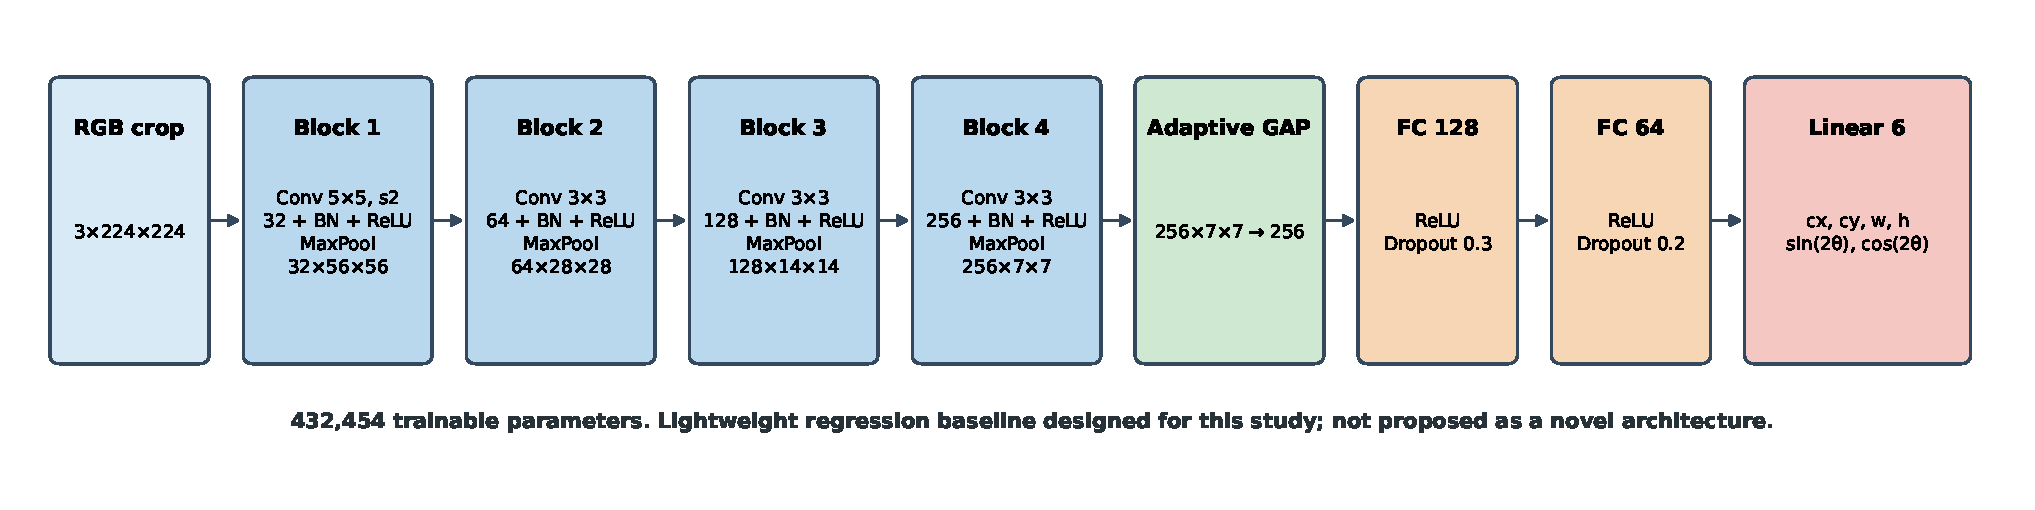
\includegraphics[width=\linewidth]{images/cnn_architecture.pdf}
  \caption{本研究用于受控比较的轻量 CNN 抓取回归结构。该完整层级安排是项目工程设计，不作为新型抓取网络贡献。}
  \label{fig:cnn-architecture}
\end{figure}

单头模型通过 128、64 单元全连接层一次输出六维；多头模型共享主干，再以中心、尺寸和方向三个分头各输出二维。两者展开形式均为
$[c_x,c_y,w,h,\sin(2\theta),\cos(2\theta)]$。双角度表示遵循 GG-CNN 的平行夹爪对称性\citep{morrison2018closing}；多头损失为三项回归损失之和，并对方向向量增加权重 0.1 的单位范数惩罚。单头共有 432,454 个可训练参数。四个块和分头方案未复制自某篇论文，而是为小数据、4\,GB GPU 和受控比较选择的轻量工程结构。

\section{共享评价与结果溯源实现}
四类感知流程把预测统一转换为中心、尺寸和方向表示，并通过共享评价模块与全部正标注比较。独立重评分器读取保存的逐样本预测，不覆盖源文件，同时输出成功见证、连续诊断、覆盖率、文件哈希和配对比较。训练代码、评价代码与图表生成读取同一 manifest 和 sample ID，使实现层的模块替换不会悄然改变评价样本。

\section{PyBullet 仿真实现}
仿真代码把场景采集、二维感知、深度反投影、候选生成、IK 与路径审计、位置控制和结果门控分为独立阶段。执行计划在发送电机命令前冻结，计划中的相机、文件哈希、抓取深度和候选高度必须一致；坐标验证和只读 preflight 不得写成物理执行。该实现结构允许第五章按依赖顺序说明实验协议，第六章再分别报告坐标、真值控制链和感知 pilot 的结果。

%==============================================================================
\chapter{实验框架}

\section{实验框架概述}
实验框架由 Cornell 离线矩形评价和 PyBullet 补充仿真两部分组成。Cornell 部分用于回答三个主要研究问题，并通过共同样本、共同裁剪、共同五折和独立重评分控制比较口径；PyBullet 部分只补充验证从二维预测到世界坐标及控制执行的接口。两部分使用不同成功判据，结果分别报告，不把离线矩形成功与仿真抬升混为同一指标。

\section{Cornell 数据集与评价划分}
实验使用 Cornell Grasping Dataset 的全部 885 幅 RGB 图像，每幅图含多个正抓取四点标注。共享加载器把四点转换为中心表示。虽然数据集包含深度，本研究统一使用 RGB，以保持输入模态不变。

历史固定目录划分以 01--06 为训练集（600 幅）、07--08 为验证集（200 幅）、09--10 为测试集（85 幅），用于配对开发阶段产物；目录号不是物体 ID，因此该划分既非标准 image-wise，也不构成 object-wise。正式补充评价使用 seed 42 生成 image-wise 五折：每折 566 幅训练、142 幅验证、177 幅测试，五个测试折合计覆盖 885 幅且每图只测试一次。共同 manifest 的 SHA-256 为
{\footnotesize\texttt{b7d3e22a145f50add6d57a70bf0abb87b4b12ee674541deab0d7fee9a286bc2d}}。Image-wise 允许同一物体的不同视角跨集合，因此只评价图像划分变化，不声称未见物体泛化。

\begin{figure}[htbp]
  \centering
  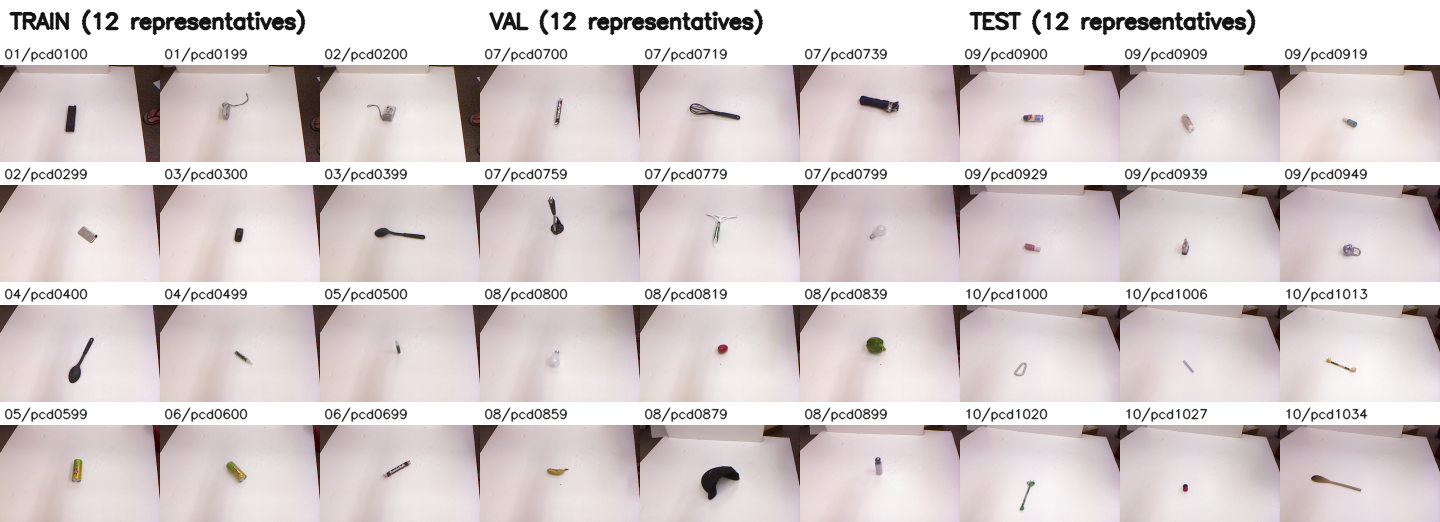
\includegraphics[width=\linewidth]{images/cornell_split_contact_sheet.png}
  \caption{训练、验证与固定测试目录中的 Cornell 示例。每个划分抽取十二幅图并尽量平衡目录；该图只展示可见物体差异，不能证明各划分难度相等。}
  \label{fig:cornell-splits}
\end{figure}

\section{训练、重复实验与交叉验证}
每幅图选择中心位于 crop 内且面积最大的正矩形作为回归目标；中心按 crop 宽高归一化，尺寸按 crop 对角线归一化。优化使用 Smooth L1、Adam、学习率 $10^{-3}$、权重衰减 $10^{-4}$、batch size 32，最多 80 epoch。ReduceLROnPlateau 在验证损失连续 8 epoch 无改善时减半学习率；20 epoch 无改善则早停并恢复最低验证损失 checkpoint。

固定目录实验对单头和多头分别运行五个随机种子 42--46，保存独立权重、历史、预测和摘要；这些目录使用旧评价器，只保留为训练过程溯源，不进入修正后的主结果。PyTorch 确定性算法、cuDNN 确定模式、固定 DataLoader generator 和关闭 benchmark 用于降低非确定性。Image-wise 五折中，两种架构读取字节相同的 manifest，各折训练 seed 固定为 42；scheduler、早停与 checkpoint 只使用 142 幅验证图，177 幅测试图不参与模型选择。Pooled 指标来自保存的 885 个折外预测按 metric-v2 独立重评分。单头与多头不仅回归头组织不同，参数量和损失构成也不同，因此比较对象是两个完整架构包，而非纯粹的单因素“分头”消融。

\section{Cornell 矩形评价}
预测 $P$ 与真值 $G$ 的交并比为
\[
\operatorname{IoU}(P,G)=\frac{|P\cap G|}{|P\cup G|}.
\]
对一幅图的全部正标注 $\{G_i\}$，rectangle success 定义为存在 $G_i$ 使 $\operatorname{IoU}(P,G_i)\geq0.25$ 且平行夹爪角度误差不超过 $30^\circ$；两个条件必须由同一个 $G_i$ 同时满足。实现另保存最大-IoU 匹配的 \texttt{best\_*} 诊断，以及使成功成立的 \texttt{successful\_match\_*} 见证。平均角度误差只对实际产生预测的样本计算，预测覆盖率单独报告，避免把缺失预测的占位角度混入质量指标。

\section{配对统计与结果审计}
四组主预测首先按 sample ID 检查唯一性与覆盖范围，再在同一图像上形成成对二元成功标签。定位前端和后端比较使用精确双侧 McNemar 检验；成功率差异、discordant pair、连续 IoU 与角度诊断分别报告，避免用单一 $p$ 值代替效应大小。五折中心值汇总全部 885 个折外预测，折间标准差只描述图像划分波动，不与五个训练 seed 的波动混用。

\section{PyBullet 补充仿真验证方法}

补充验证分为两层：第一层关闭从二维抓取中心到目标表面世界点的数据流缺口；第二层以真值姿态验证完整运动-接近-闭合-抬升控制链后，加载由感知生成的冻结执行计划，在相同仿真环境中驱动完整物理抓取。

\subsection{坐标反投影验证}
采用一个固定 PyBullet 场景，其中包含黄色鸭、红色方块、绿色球体和作为干扰项的 Franka Panda。三条明确目标提示和 geometry、single、multi-head 三个后端复用同一幅 $640\times480$ RGB 图像、米制深度、segmentation、view matrix 与 projection matrix。只有正确选择目标后保存的九个二维抓取中心进入坐标验证；该过程发生在二维预测之后，不改变 Grounding DINO 或三个后端的输入。

对每个中心 $(c_x,c_y)$，系统采用最近像素并以 half-up 规则取整得到列与行，然后读取该像素的米制深度。米制深度先按 PyBullet/OpenGL 透视深度关系还原为 depth-buffer 值，再使用列主序 projection matrix 的逆矩阵恢复相机齐次坐标，并使用 projection--view 组合矩阵的逆矩阵恢复世界坐标。所得世界点随后通过原 view/projection matrix 重投影到图像。相机矩阵和深度缓冲约定遵循 \href{https://github.com/bulletphysics/bullet3/blob/master/docs/pybullet_quickstartguide.pdf}{Bullet Physics 官方 PyBullet Quickstart Guide}。

逐点门控要求深度严格位于 $0.05$\,m 与 $3.0$\,m 裁剪面之间、全部相机与世界坐标有限、像素重投影误差不超过 $1$\,px、深度往返误差不超过 $10^{-4}$\,m、采样像素的 segmentation body 与指定目标一致，且从相机光心穿过反投影点并延长 $0.05$\,m 的 \texttt{rayTest} 首次命中同一目标。Segmentation 与射线结果只在坐标产生后作真值审计。

\subsection{真值姿态分阶段控制链验证}
在加载感知预测之前，先用固定 cube 真值位姿逐阶段验证 Panda 位置电机控制链的可行性。场景含桌面、Franka Panda（自碰撞开启）和作为目标的红色方块（半高 $0.025$\,m），固定随机种子 42。

各阶段按依赖顺序递增实现。阶段 1：从中立位姿执行安全空中往返（$0.05$\,m 上升后返回），验证 \texttt{POSITION\_CONTROL} 与 \texttt{stepSimulation} 链路，手指保持 $0.04$\,m 张开。阶段 2：使用真值 AABB 顶面生成俯视 pregrasp（表面上方 $0.12$\,m），到达后记录末端-方块相对位置。阶段 3：从 pregrasp 沿世界 Z 下降 $0.10$\,m 到达接触前高度（顶面上方 $0.02$\,m），手指保持张开。阶段 4：增加 $0.015$\,m 短下探至顶面上方 $0.005$\,m 后缓慢闭合双指，首次双指同时产生目标正法向力时冻结命令并保持 120 步；审计非手指目标接触、其他环境接触和自碰撞。阶段 5：冻结阶段 4 的最终双指命令，沿世界 Z 抬升 $0.12$\,m 后保持 240 步；审计方块上升量、桌面接触、工具-方块相对漂移、双指法向力和禁止碰撞。每个阶段仅增加一种能力，不跨越未验证的门控。

各阶段均审计到达位置误差（$\leq 5$\,mm）、方向误差（$\leq 5^\circ$）、方块最大位移（$\leq 0.001$\,m）、双指张开误差（$\leq 0.001$\,m）、关节终点误差（$\leq 0.01$\,rad）和碰撞计数（环境 $=0$，自碰撞 $=0$）。阶段 4/5 额外审计双指接触连续步数与法向力。只有全部门控通过才进入下一阶段，只有阶段 5 通过才计为一次真值姿态仿真抓取成功。

\subsection{感知预检与执行计划生成（Stage 6A）}
在同一固定场景中，稳定 60 步后采集一帧 $640\times480$ RGB 图像，运行 \path{IDEA-Research/grounding-dino-tiny}（提示 \texttt{red cube}）定位目标，由 geometry 后端在定位框内产生二维抓取矩形。抓取中心按单像素最近深度反投影为世界表面点，随后生成两个对称（$0^\circ/180^\circ$）俯视悬停候选，各含 pregrasp（表面上方 $0.10$\,m）、approach（表面上方 $0.02$\,m）和 grasp\_depth（表面上方 $0.005$\,m）三个位姿。每个候选经七关节 IK 求解、FK 验证（$\leq 5$\,mm、$\leq 5^\circ$）和路径碰撞审计（两阶段：接触前含目标、抓取深度排除预期目标，各 41 个采样状态，余量 $0.002$\,m）。通过审计的候选按低关节代价值确定性地选择 $0^\circ$。全部感知证据、审计结果和冻结执行计划写入 \path{execution_plan.json}；该阶段不发送电机命令。

\subsection{中心偏差诊断与恢复尝试（Stage 6A.1/6A.2）}
使用冻结的 cube 真值位姿和半高 $0.025$\,m 对 Stage 6A 产物进行只读后验审计：预测世界表面点相对 cube 质心的 X/Y 偏差为 $0.026/0.002$\,m（XY 合成 $0.0266$\,m），不满足 $0.005$\,m 参考门槛；Z 偏差为 $0.0005$\,m。诊断在独立目录完成真实 CUDA 重跑验证，RGB 哈希、定位框和偏差值一致。随后尝试窗口化（$5\times5$）目标 mask 最小深度恢复：对 geometry 和 multi-head 共同应用同一规则，但 geometry XY 偏差升至 $0.0276$\,m，multi-head 升至 $0.0264$\,m。该方案被排除，选择冻结为回退至原始单像素反投影。

\subsection{感知驱动完整物理抓取（Stage 6B）}
加载 Stage 6A 冻结执行计划，直接使用计划中的预计算 IK 解和感知位姿驱动七阶段抓取链条：中立位→pregrasp→approach→grasp\_depth→闭合→接触保持→抬升→保持。除位姿源来自感知而非真值外，所有运动控制参数、门控门槛和审计流程与真值阶段 2-5 相同。执行前重跑两阶段路径碰撞审计（接触前含 cube、抓取深度排除 cube）和抬升路径审计。Stage 6B 同样以 geometry 和多头 CNN 分别执行，形成配对物理证据。该阶段是本文 PyBullet 仿真中第一次用感知输出（而非真值坐标）驱动完整机械臂运动；全部运动、接触和抬升标志为真。

\subsection{头顶相机与深抓取联合干预（Stage Overhead）}
为考察斜视 Stage 6B 中的 XY 中心偏差，增设头顶（overhead）相机 preflight。相机置于场景正上方（$\textit{eye}=(0.5,0.0,1.3)$，$\textit{target}=(0.5,0.0,0.62)$），光轴垂直向下；采用 $\textit{up}=(0,1,0)$ 以避免标准 $\textit{up}=(0,0,1)$ 与视线平行导致的 view matrix 退化。感知管线仍使用 Grounding DINO（提示 \texttt{red cube}）、geometry 二维抓取和单像素深度反投影，不启用中心恢复。

该运行还把 grasp\_depth standoff 从 $+0.005$\,m 改为 $-0.025$\,m，使 TCP 下探至 cube 中心高度；approach 保持 $+0.020$\,m，候选 pregrasp 位于 approach 上方 $0.100$\,m。首次尝试 $-0.060$\,m 因桌面碰撞未通过，$-0.025$\,m 的候选通过静态审计。完整性复核发现，历史 JSON 虽携带 $-0.025$\,m 候选，却仍声明冻结的 $+0.005$\,m 控制。当前实现已将这组值冻结为独立协议 \texttt{stage\_6a\_overhead\_deep\_grasp\_v1}，并强制 world surface point、control offset 与候选 Z 高度一致；历史不一致计划会被严格加载器拒绝。

历史头顶计划随后执行了完整物理抓取并成功抬升。因为相机位姿和抓取深度同时变化，且计划元数据存在上述不一致，这一结果是联合干预的固定场景 $N=1$ 可行性证据，不是控制变量相机对照。严格新协议的 preflight 与 Stage 6B 仍需重新运行；若要分离因果作用，需要补做“斜视/顶视 $\times$ $+5/-25$\,mm”二乘二实验。

\section{可复现性与研究伦理（Research Ethics）}
本项目无人类参与者、问卷或私人数据，不涉及知情同意与个人保密。Cornell 数据和公开预训练模型仅用于学术研究；相关论文、外部模型和任何引用或改编代码均应标明出处，项目自写结构不冒充文献方法。结果只从保存的 JSON、CSV 和预测产物写入论文，不把定位覆盖率夸大为定位质量，也不把离线矩形成功夸大为机器人成功。随机种子、环境版本、manifest 哈希和确定性设置支持审计；冻结大型 VLM、限制轻量后端和重复次数也控制了计算资源消耗。

\section{实验设计局限}
固定目录接触图不能证明难度相等；image-wise 五折仍可能有相邻视角信息泄漏。由于现有文件缺少可审计的 885 图像到物体实例映射，本文不报告 object-wise。Grounding DINO 可能对 prompt 和阈值敏感，但本研究未做提示搜索。CNN 只用小规模 RGB crop 并输出单矩形，而现代方法常利用 RGB-D 与密集多抓取图。Cornell 的最终评价仍是 RGB-only offline metric；PyBullet 补充验证中的坐标反投影仅恢复目标表面点，完整物理抓取限于单场景 $N=1$，均不等同于真实机器人抓取成功率。

%==============================================================================
\chapter{实验方案与结果}

本章按“实现与数据审计、三个研究问题、补充仿真、定性案例”的顺序报告结果。所有 Cornell 主数字来自保存预测的 metric-v2 独立重评分；PyBullet 结果遵循第五章的分阶段门控并保持独立证据边界。

\section{数据与实现验证}
数据审计确认训练、验证和固定测试目录分别含 600、200 和 85 幅图，总数为 885。随机抽查原图、正抓取叠加图和图~\ref{fig:cornell-splits} 后，图像与标注 ID 对齐。传统整图基线有 55 幅图未产生轮廓抓取；保存的 Grounding DINO 运行对 885/885 幅图返回有效框，两个 VLM 引导流程均产生抓取矩形。这里的 885/885 只验证输出覆盖完整，不能说明框紧密包围物体，更不能单独证明定位或抓取正确。

历史 metric-v1 固定目录记录显示，传统非学习基线在 600 幅训练图上的成功率低于 85 幅测试目录，提示目录 09--10 可能对当前颜色与轮廓规则更容易。由于该表未逐 seed 按 metric-v2 重建，它只作为划分偏置警告，不进入修正后的结果比较。

结果写入前还进行了文件级溯源。四组源预测各覆盖 885 个唯一 sample ID（传统 CV 中 55 行明确记录无预测）；image-wise 的每个架构各保存五份测试预测，合并后均为 885 个互不重复 ID，两个架构记录的 manifest 哈希一致。独立重评分器不覆盖源 CSV，并把源/输出 SHA-256、成功见证与配对检验写入 \path{data/processed/shared/cornell_metric_v2/summary.json}；该总摘要 SHA-256 为 {\footnotesize\texttt{6ed8d6cf3d621f2f\allowbreak{}a9171edfe1db0fc\allowbreak{}8af1d6d684c287f4\allowbreak{}b8565219128c6d02f}}。该验证保证统计过程可追溯，不替代对算法有效性的分析。

\section{研究问题一：开放词汇定位的作用}
表~\ref{tab:main-results} 使用修正后的 metric-v2 比较四组保存预测。传统 CV 成功 522/885（58.98\%），VLM + geometry 成功 659/885（74.46\%），绝对增加 137 个样本与 15.48 个百分点。逐样本配对中二者共同成功 513、共同失败 217、仅 CV 成功 9、仅 geometry 成功 146；精确双侧 McNemar 检验 $p=5.24\times10^{-33}$。因此，在当前实现与样本上，加入 Grounding DINO 处理范围与明显改善相关。

传统 CV 只为 830/885 图像产生预测，覆盖率 93.79\%；其条件角度误差 19.65$^\circ$ 只对这 830 个预测求均值。Geometry 的预测覆盖率为 100\%，条件角度误差 14.81$^\circ$。Grounding DINO 的 885/885 返回框同样只表示 detection coverage；没有逐框真值定位评价，不能把主表差异解释为通用 VLM 定位精度或唯一机制。

\begin{table}[htbp]
  \centering
  \caption{Cornell metric-v2 主结果。CNN 为 885 条 image-wise 五折折外预测；角度只对实际预测求均值，覆盖率单列。}
  \label{tab:main-results}
  \resizebox{\linewidth}{!}{%
  \begin{tabular}{lrrrrr}
    \toprule
    方法 & 成功数 & 成功率 & 平均最佳 IoU & 条件角度误差 & 覆盖率 \\
    \midrule
    传统 CV 基线 & 522/885 & 58.98\% & 0.3360 & $19.65^\circ$ & 93.79\% \\
    VLM + 几何后端 & 659/885 & 74.46\% & 0.4182 & $14.81^\circ$ & 100\% \\
    VLM + 单头 CNN（OOF） & 661/885 & 74.69\% & 0.4390 & $17.74^\circ$ & 100\% \\
    VLM + 多头 CNN（OOF） & 671/885 & 75.82\% & 0.4580 & $17.40^\circ$ & 100\% \\
    \bottomrule
  \end{tabular}}
\end{table}

\section{研究问题二：几何与 CNN 后端比较}
折外结果使几何与学习后端可以在相同 885 个 sample ID 上配对。Geometry 与单头 CNN 的成功率只差 0.23 个百分点；discordant pair 为 88/90，精确 McNemar $p=0.940$。Geometry 与多头 CNN 相差 1.36 个百分点；discordant pair 为 77/89，$p=0.393$。两项检验均不支持二元成功率差异显著。

连续诊断显示不同取舍：单头/多头平均最佳 IoU 为 0.4390/0.4580，高于 geometry 的 0.4182；geometry 的条件角度误差 14.81$^\circ$，低于单头/多头的 17.74$^\circ$/17.40$^\circ$。这些结果支持“学习后端空间重合较高、显式几何方向先验较低误差”的描述，但不能推出某个后端在总体上严格支配另一个。旧固定 85 样本与五-seed 目录尚未按 metric-v2 逐 seed 重建，故不再作为主证据。

\section{研究问题三：单头与多头 CNN 比较}
表~\ref{tab:image-wise-cv} 使用字节相同的 image-wise manifest。单头的 885 个折外预测成功 661 个（74.69\%），多头成功 671 个（75.82\%）；多头增加 10 次成功，即 $+1.13$ 个百分点。配对表为共同成功 615、共同失败 168、仅单头成功 46、仅多头成功 56，精确 McNemar $p=0.373$。因此不能拒绝二者二元成功率相同的零假设。

\begin{table}[htbp]
  \centering
  \caption{Image-wise 五折结果。中心值汇总 885 个折外预测，$\pm$ 为五个等大测试折之间的总体标准差。}
  \label{tab:image-wise-cv}
  \resizebox{\linewidth}{!}{%
  \begin{tabular}{lrrrr}
    \toprule
    架构 & 成功数 & 成功率 & 平均最佳 IoU & 平均角度误差 \\
    \midrule
    单头 CNN & 661/885 & $74.69\%\pm2.85\%$ &
      $0.4390\pm0.0190$ & $17.74^\circ\pm1.23^\circ$ \\
    多头 CNN & 671/885 & $75.82\%\pm3.24\%$ &
      $0.4580\pm0.0191$ & $17.40^\circ\pm1.13^\circ$ \\
    \bottomrule
  \end{tabular}}
\end{table}

这里的 $\pm$ 是修正后五个等大测试折成功率的总体标准差，不是五个训练 seed 的波动。单头逐折成功数为 135、124、129、138、135，多头为 128、132、129、142、140；多头在 fold 0 少 7 次、fold 2 相同，其余三折较高，说明差异并非每折一致。多头平均最佳 IoU 高 0.0190，条件角度误差低 0.34$^\circ$，但这些连续差值未在本研究中做配对显著性检验。再加上两种模型参数量（432,454 与 514,758）和损失构成不同，研究问题三只能回答为“当前多头架构包有小幅描述性优势，证据不足以声称显著或归因于分头本身”。

\section{补充 PyBullet 仿真验证}

\subsection{坐标反投影门控}
固定 PyBullet 场景沿用前述三条明确提示，三个目标均被正确选择（3/3），平均指定目标 IoU 为 0.8600；这两个数值只用于说明九点坐标验证的上游条件。Geometry、single 与 multi-head 各为鸭、方块和球体产生一个二维中心，形成按目标和后端固定排序的九条记录。表~\ref{tab:pybullet-backprojection} 汇总坐标门控；全部九条均具有有限坐标和有效米制深度，重投影、segmentation 目标匹配与射线目标匹配也均通过。

\begin{table}[htbp]
  \centering
  \caption{固定单场景的九点 PyBullet 坐标集成门控。该表验证二维中心到目标表面世界点的数据流，不是物理抓取成功率，也不用于比较后端性能。}
  \label{tab:pybullet-backprojection}
  \begin{tabular}{lcl}
    \toprule
    检查项 & 结果 & 判据或用途 \\
    \midrule
    有限坐标 & 9/9 & 所有相机与世界坐标有限 \\
    有效米制深度 & 9/9 & $0.05\,\mathrm{m}<d<3.0\,\mathrm{m}$ \\
    重投影门控 & 9/9 & $\leq1$\,px 且 $\leq10^{-4}$\,m \\
    segmentation 目标匹配 & 9/9 & 事后真值审计 \\
    \texttt{rayTest} 目标匹配 & 9/9 & 事后真值审计 \\
    总门控 & 通过 & 九条顺序完整且逐点通过 \\
    \bottomrule
  \end{tabular}
\end{table}

九点中的最大像素重投影误差为 $8.04\times10^{-13}$\,px，最大深度往返误差为 $3.57\times10^{-7}$\,m，均远低于预先固定的工程门槛。反投影点到射线实际命中位置的最大距离为 $0.00676$\,m；该值受渲染深度表面与碰撞几何差异影响，只作为诊断量。九条记录来自同一确定性场景和同一图像，不能据此计算成功率或后端排序。

\subsection{真值姿态控制链验证}
表~\ref{tab:truth-control-chain} 汇总五个分阶段验证结果。阶段 1 完成中立位→安全点→中立位的空中往返（506 步），末端位置误差 $0.0005$\,m。阶段 2 使用真值 AABB 顶面到达 pregrasp，末端-方块 XY 偏差 $0.0007$\,m。阶段 3 张手下降至接触前高度，实际工具高度与计划 $0.02$\,m 的误差为 $0.0008$\,m。阶段 4 增加短下探后闭合双指，在闭合第 93 步首次同时接触并保持。当前阶段 5 产物记录 3591 个状态；方块最终上升 $0.120005$\,m（门槛 $0.10$\,m），保持段桌面接触为零，全程 1 次，末端--方块最大相对漂移 $0.002142$\,m（门槛 $0.01$\,m）。全部门控通过，阶段 5 计为一次真值姿态仿真抓取成功。

\begin{table}[htbp]
  \centering
  \caption{真值姿态分阶段控制链验证结果。每阶段只增加一种新能力，通过后才进入下一阶段。}
  \label{tab:truth-control-chain}
  \resizebox{\linewidth}{!}{%
  \begin{tabular}{lcccc}
    \toprule
    阶段 & 步数 & 关键指标 & 测得值 & 判据 \\
    \midrule
    1 安全运动 & 506 & 末端位置误差 & $5.1\times10^{-4}$\,m & $\leq5$\,mm \\
    2 pregrasp & 267 & 末端-方块 XY 偏差 & $6.6\times10^{-4}$\,m & $\leq5$\,mm \\
    3 开放接近 & 522 & 接触前高度误差 & $7.7\times10^{-4}$\,m & --- \\
    4 双指接触 & 975 & 首次接触步/保持步 & 93 / 121 & --- \\
    5 抬升保持 & 3591 & 方块上升/漂移 & 0.120005\,m / $2.14\times10^{-3}$\,m & $\geq0.10$\,m / $\leq0.01$\,m \\
    \bottomrule
  \end{tabular}}
\end{table}

\subsection{感知预检与中心偏差诊断}
Geometry 的 Grounding DINO 定位框为 $[297,189,344,245]$、分数 $0.8170$、cube IoU $0.8717$。二维抓取中心、角度、单像素深度和反投影世界点分别为
\[
(320.5,217.0),\qquad 0^\circ,\qquad 0.6838\,\mathrm{m},\qquad
(0.5065,0.0022,0.6755)\,\mathrm{m}.
\]
两个对称候选均通过 82 状态两阶段碰撞审计，确定性选择 $0^\circ$；静态科学门控通过。然而，使用保存的 cube 真值质心 $(0.48,0.0,0.65)$\,m 和冻结半高 $0.025$\,m 进行后验审计后发现：预测世界点相对质心的 X/Y 偏差为 $0.0265/0.0022$\,m，XY 合成偏差 $0.0266$\,m（$26.55$\,mm），不满足 $0.005$\,m 参考门槛；Z 偏差仅为 $0.0005$\,m。独立 CUDA 重跑确认 RGB 哈希、定位框和偏差值一致。

\subsection{中心恢复尝试}
对 geometry 和 multi-head 共同应用窗口化（$5\times5$）目标 mask 最小深度恢复后，geometry XY 偏差升至 $0.0276$\,m（$27.60$\,mm），multi-head 升至 $0.0264$\,m（$26.43$\,mm）。两后端静态门控均通过，但 XY 偏差无一下降。分析确认：斜视相机（位于 $X=1.0$\,m）观测 $X=0.48$\,m 处的 cube 时，窗口内最小深度自然选中朝向相机的边缘，进一步将世界点拉向 $+X$ 方向，恶化中心偏差。该方案被排除，后续回退至原始单像素反投影。

\subsection{感知驱动完整物理抓取}
表~\ref{tab:perception-grasp-results} 对比真值抬升与两个后端的感知物理抓取结果。Geometry 与 multi-head 的 pregrasp、approach 和 grasp\_depth 到达位置误差均在 $1.04$\,mm 以内，全部通过动态门控。夹爪闭合并建立双指接触（geometry 首次接触在闭合第 226/240 步，multi-head 在 218/240 步，远晚于真值的 93 步），接触保持均达 120 步。然而，两个后端在抬升阶段均失败：cube 仅上升 $0.38$\,mm（geometry）和 $0.34$\,mm（multi-head），远低于 $0.10$\,m 门槛；末端-cube 相对漂移均达 $0.12$\,m（与抬升命令量相等，表明 cube 完全未动）；桌面接触各 481 次。夹爪虽闭合但仅触及 cube 边缘，抬升时立即滑脱。

\begin{table}[htbp]
  \centering
  \caption{真值抬升与两个历史感知 pilot 的结果。两个感知运行均有较大 XY 偏差并在抬升阶段失败；该共现不是唯一根因证明。}
  \label{tab:perception-grasp-results}
  \begin{tabular}{lccc}
    \toprule
    指标 & 真值（阶段 5） & Geometry（Stage 6B） & Multi-head（Stage 6B） \\
    \midrule
    XY 偏差 & $\approx0$\,mm & $26.62$\,mm & $24.67$\,mm \\
    pregrasp 到达误差 & $0.95$\,mm & $1.04$\,mm & --- \\
    approach 到达误差 & $0.78$\,mm & $0.78$\,mm & --- \\
    grasp\_depth 到达误差 & --- & $0.63$\,mm & --- \\
    首次双指接触步 & 93 & 226 & 218 \\
    接触保持步 & 121 & 120 & 120 \\
    Cube 最终上升 & $0.120$\,m & $0.0004$\,m & $0.0003$\,m \\
    末端-cube 漂移 & $0.0021$\,m & $0.120$\,m & $0.120$\,m \\
    抬升桌面接触 & 1 & 481 & 481 \\
    科学门控 & 通过 & 失败（抬升） & 失败（抬升） \\
    \bottomrule
  \end{tabular}
\end{table}

两个后端都出现超过约一个 cube 半宽的 XY 偏差并在抬升阶段失败，这与“单像素可见表面点不是物体中心，导致边缘接触”的解释一致。相似结果提示共享前端问题，但每个后端只有一次固定场景运行，没有重复配对或控制消融，因而不能排除其他共同控制因素，也不能证明问题完全只在 XY 平面。

\subsection{历史头顶 + 深抓取联合 pilot}
历史头顶运行的 XY 中心偏差为 $0.76$\,mm，且成功抬升。表~\ref{tab:overhead-grasp} 将它与斜视 geometry pilot 并列，但两者至少有两个变化：相机位姿，以及 grasp standoff 从 $+5$\,mm 到 $-25$\,mm。后者直接改变夹爪相对 cube 的接触高度，因此不能把结果差异归因于相机单因素。

\begin{table}[htbp]
  \centering
  \caption{斜视标准抓取与历史头顶深抓取 pilot。相机与抓取深度同时变化，故该表不是单因素对照。}
  \label{tab:overhead-grasp}
  \begin{tabular}{lcc}
    \toprule
    指标 & 斜视相机（Stage 6B） & 头顶相机（Stage 6B） \\
    \midrule
    XY 中心偏差 & $26.55$\,mm & $0.76$\,mm \\
    Grasp standoff & $+5$\,mm & $-25$\,mm \\
    pregrasp 到达误差 & $1.04$\,mm & $\leq1.0$\,mm \\
    approach 到达误差 & $0.78$\,mm & $\leq1.0$\,mm \\
    grasp\_depth 到达误差 & $0.63$\,mm & $\leq1.0$\,mm \\
    首次双指接触步 & 226 & 41 \\
    接触保持步 & 120 & 120 \\
    Cube 最终上升 & $0.0004$\,m & $0.1199$\,m \\
    末端-cube 漂移 & $0.120$\,m & $0.0014$\,m \\
    抬升桌面接触 & 481 & 2 \\
    历史科学门控 & 失败（抬升） & 旧实现通过 \\
    \bottomrule
  \end{tabular}
\end{table}

历史头顶运行中，到达误差均不超过 1.0\,mm，双指首次接触在闭合第 41 步，cube 最终上升 $0.1199$\,m，末端--cube 漂移 $0.0014$\,m。该输出证明联合配置在这个固定场景可以工作。然而旧计划把 $-25$\,mm 候选错误声明为冻结 $+5$\,mm 控制，当前严格加载器会拒绝它；新增的真实抓取深度高度门控也尚未在新计划上运行。因此论文不把旧 \texttt{scientific\_gate} 作为新协议验证，也不声称完成了相机因果闭环。

\section{定性案例与失败分析}
图~\ref{fig:backend-failures} 保留了固定目录开发阶段的代表矩形，用于观察中心、尺度、方向和 VLM 框宽松度。绿色为 Cornell 正标注，黄色为 VLM 框，蓝色为保存的 seed 46 单头预测，红色为 geometry 预测。该图按旧 metric-v1 标签选样，不能再支持 CNN-only/geometry-only 的数量结论；修正后的定量比较只使用表~\ref{tab:main-results} 的 OOF 结果与配对检验。

\begin{figure}[htbp]
  \centering
  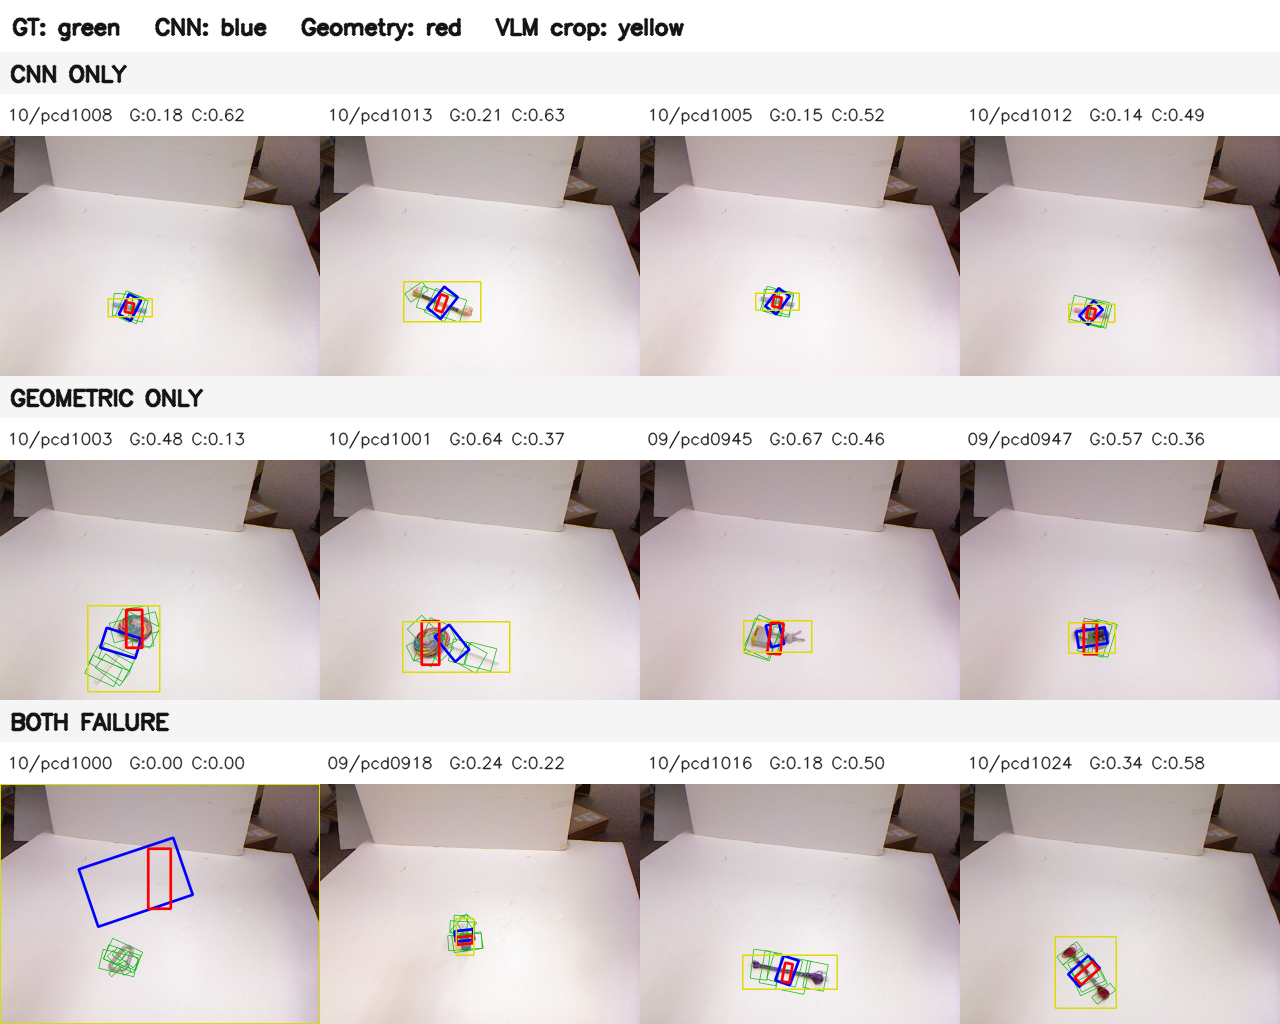
\includegraphics[width=\linewidth]{images/backend_failure_cases.png}
  \caption{固定目录开发阶段的代表矩形。选样标签来自历史 metric-v1，因此该图只展示几何现象，不估计类别频率或后端胜负。}
  \label{fig:backend-failures}
\end{figure}

部分蓝色矩形在中心或尺度上更接近正标注，部分红色矩形的方向更接近标注；这与 OOF 的平均 IoU/角度诊断方向一致，但图片本身不能证明模型学会了特定部位或某种先验产生了因果收益。宽松 VLM crop、单目标多解标注、尺寸回归和方向边界均仍可能参与误差。

边界案例还揭示二值阈值的限制。接近 IoU 0.25 或 $30^\circ$ 的矩形只需轻微变化就会翻转标签，因此正文同时保留连续指标、覆盖率和成功见证。后续若重新生成定性类别，必须直接读取 metric-v2 成功字段，而不能从最大-IoU 诊断单独反推成功。

\section{结果小结}
三个研究问题得到层层收窄的证据。第一，加入开放词汇定位后，既定几何流程相对整图 CV 增加 15.48 个百分点，配对差异清晰。第二，共同 crop 下 CNN 的平均最佳 IoU 较高、geometry 条件角度误差较低，但 geometry 与两个 OOF CNN 的二元成功率配对差异均不显著。第三，多头相对单头只增加 1.13 个百分点，$p=0.373$，只能报告描述性差异。

这些结果的可辩护范围是 Cornell RGB 单目标、通用提示、当前实现与离线 rectangle metric。主结果使用独立重评分的 OOF/全量保存预测；旧五 seed 与固定 85 样本表不进入 metric-v2 主张。结果不证明对未见物体、杂乱开放世界或真实机器人执行的同等增益。

补充 PyBullet 结果按依赖顺序提供三类证据：九点坐标数据流、一次真值姿态控制链成功，以及若干固定场景感知 pilot。两个斜视后端均有大 XY 偏差并抬升失败；历史顶视 + 深抓取联合配置偏差较小并抬升成功。由于两个变量同时改变且旧计划控制声明不一致，最后一项只证明联合配置可行。它们不是正式重复试验，不能计算感知成功率、后端排名或相机因果效应。

%==============================================================================
\chapter{结果总览与讨论}

\section{结果总览}
整体证据呈现清晰但有限的层次：开放词汇定位带来的几何流程改进最大且配对差异明确；共同 crop 下，几何与 CNN 分别在方向和空间重合诊断上占优；多头相对单头只有小幅描述性提升且缺少显著性支持。PyBullet 补充实验关闭了坐标与控制接口的一部分缺口，但当前感知执行仍是固定单场景 pilot，不能转化为后端排名或相机因果结论。

\section{主要发现的解释}
最明显的变化来自加入定位范围：保持颜色、轮廓和几何规则基本相同，把整图处理限制到 Grounding DINO 区域后，metric-v2 成功率增加 15.48 个百分点，55 个缺失预测降为零。一个合理解释是 VLM crop 排除了部分背景和干扰轮廓，但本研究没有人工框上限、框定位准确率或强任务专用检测器对照，所以不能断言 VLM 是唯一机制或必要方案。

CNN 与几何的诊断优势落在不同维度。单头和多头 CNN 的平均最佳 IoU 较高，geometry 的条件角度误差较低。多头相对单头的 pooled 差异为 1.13 个百分点，且 $p=0.373$；参数量与损失也不同。因此数据只支持完整架构包之间的小幅描述性差异，不支持“分头结构显著更好”的结论。

不同连续指标仍可提出“学习中心和尺度、用几何约束方向”的混合后端假设，但当前实验未实现该消融。固定目录历史结果还提示测试子集偏易，所以无论如何都不能解释为 object-wise 泛化。

\section{与既有文献的关系}
本项目沿用 Jiang 的二维矩形和 Cornell 判定框架\citep{jiang2011efficient}。Lenz 的 RGB-D 两阶段候选评分展示了深度特征与候选重排的价值，并同时报告 image-wise/object-wise\citep{lenz2015deep}；Redmon 则把搜索改为全局直接回归和网格多抓取\citep{redmon2015real}。本研究的轻量 CNN 与 Redmon 同属“图像到矩形”范式，但输入是 Grounding DINO 产生的 RGB crop，fold 成员也由本项目生成，因此数值只能有限可比。

GG-CNN 以深度图密集预测质量、方向和宽度\citep{morrison2018closing}，GR-ConvNet 与 Gaussian-guided 网络继续发展像素级多抓取输出\citep{kumra2020antipodal,li2022gaussian}。这些方法能保留多个局部候选，表达力高于本项目的单矩形回归；同时使用深度、增强和不同协议。它们的高 Cornell 数字用于说明技术方向，而不能与当前 RGB-only 结果直接形成排行榜。其物理实验还包含标定、运动、接触与恢复，Cornell rectangle success 不等同于物理抓取成功。

Grounding DINO 的原始贡献是文本条件开放集检测\citep{liu2023grounding}，本项目只把它当作可替换定位前端，而不把它称为抓取模型。Vuong 的 Language-driven Grasp Detection 在复杂场景中用具体语言指令条件化生成抓取\citep{vuong2024language}；当前实验对所有单目标图固定 \texttt{small object}，没有测试语言指定部位或多目标消歧。两者共享“语言参与目标选择”的动机，但任务、数据和评价均不同。

\section{失败案例与误差来源}
Metric-v2 下 VLM + geometry 有 226 个失败。其中 191 个样本的最大 IoU 仍低于 0.25，表示没有标注达到空间门槛；其余 35 个至少有标注达到 IoU 门槛，但没有同一标注同时通过角度门槛。该两类划分比旧的“仅 IoU/仅角度/两者”分类更符合存在性判据，但仍是观测诊断，不是原因标签。Grounding DINO 的 100\% detection coverage 只表示每图返回框；宽松、偏移或错误框仍可能计入覆盖。

旧固定目录案例图可以提示尺度、中心、方向和框宽松度问题，却不能沿用旧 success 标签进行频率统计。后续案例分析应直接从 metric-v2 CSV 读取成功见证，并对同一 GT 的 IoU/角度组合进行可视化；在该分析完成前，不从少量图片推断总体因果比例。

\section{实践与理论意义}
工程上，开放词汇检测器可以作为可替换模块缩小轻量抓取估计器的搜索区域，尤其适用于类别名称变化或缺少封闭集检测器的场景。共享 crop 也使后端可以独立升级。结果同时提示不应丢弃简单几何信息：学习回归与解析方向先验解决不同样本，混合方案值得正式消融。

理论上，本研究支持模块化误差观：语言 grounding 处理“选择哪个区域”，抓取后端处理“该区域怎样夹持”。Detection coverage 与 grasp affordance 不等同；VLM 可以改善当前感知管线，却没有因此自动获得接触力学、可达性或碰撞知识。

若进入部署，还需在当前单点反投影基础上确定抓取方向与预抓取姿态，并完成相机到机器人标定、轨迹生成、近距离重估、夹爪闭合和成功检测。当前感知与坐标输出应被视为这些阶段的输入，而非完整机器人系统。

\section{从感知到物理执行的补充证据}
PyBullet 补充验证按依赖顺序构建了三层证据，对应三维抓取的不同门控层级。第一层（坐标反投影）确认二维中心、米制深度和相机矩阵能够在当前实现中产生数值有限、可重投影且命中指定目标的世界点；9/9 首先验证的是软件数据流、矩阵顺序、图像坐标方向和深度换算约定。第二层（真值控制链）证明当前 Panda 仿真环境中，从 IK 求解、路径碰撞审计、位置电机执行到夹爪闭合和抬升保持的完整链路均可工作，且每个阶段只在前一阶段通过后才增加新能力。第三层（感知驱动执行）将前两层合并：使用感知生成的冻结计划和预计算 IK 解驱动同一链条后，静态和到达门控全部通过，但抬升因 XY 中心偏差失败。

这一分层设计缩小了解释空间：真值链成功说明仿真控制至少在一个中心对准的运行中可行，两个斜视感知运行的失败则与共享的表面点偏差假设一致。但“相似失败”不能排除其他共同因素。更重要的是，历史头顶运行不仅改变相机，还把 grasp standoff 从 $+5$\,mm 改为 $-25$\,mm；旧计划又没有如实编码该控制。因此 $26.55\rightarrow0.76$\,mm 与 $0.0004\rightarrow0.1199$\,m 的同时变化不能构成相机因果闭环。当前最强结论是联合配置在固定场景可行；分离相机与抓取深度需要二乘二消融，后端比较需要同控制重复配对。

\section{研究局限}
第一，研究只用 Cornell 小型单物体数据，不能代表杂乱开放世界。第二，Cornell 训练与评价输入保持 RGB-only；补充 PyBullet 验证中的单像素反投影仅使用单个深度样本恢复表面点，未利用局部深度结构（如法向估计）改进三维定位。第三，image-wise 允许相邻视角跨集合，权威物体映射缺失使 object-wise 暂不可审计。第四，固定 85 样本较小且难度偏置明显。第五，通用 prompt、框阈值和 10\% 扩张未做敏感性实验，885/885 定位覆盖率也不是定位质量。

第六，几何与 CNN 都只输出单矩形，不能表示一物多抓取。第七，仿真物理抓取限于单场景 $N=1$、单物体和固定夹爪/物体几何，无真实机器人验证；边缘抓取在更宽夹爪或更大物体上可能偶然成功。第八，各 fold 只有 566 幅训练图，4\,GB GPU 限制模型容量与搜索范围；五 seed 和 fold 统计均显示非零波动。因此，当前 CNN 应被理解为受控轻量基线，多头结果是局部证据，而非最新方法或最终架构。

%==============================================================================
\chapter{结论与未来工作}

\section{研究总结}
本论文研究开放词汇定位如何作为二维机器人抓取检测的前端。针对既有文献在 RGB/RGB-D、数据划分和输出形式上难以直接比较的问题，研究在 Cornell 的 885 幅 RGB 图像上构建整图传统 CV、VLM + geometry、VLM + 单头 CNN 和 VLM + 多头 CNN，并用共同标注、固定目录、五个随机种子及共同 image-wise 五折区分定位贡献、训练波动与架构差异。评价同时保留 rectangle success、IoU、角度误差和逐样本案例。

论文的核心发现不是某个模型在所有条件下最优，而是不同模块和指标需要分开审计。定位范围带来最大的测得差异；学习后端的平均 IoU 较高，几何后端的角度诊断较低；多头与单头的成功率差异则没有统计支持。连续指标、覆盖率、配对检验和成功见证共同防止二元成功率掩盖角度、尺度或缺失预测。

\section{研究问题回答}
\textbf{研究问题一：}在当前 Cornell RGB、通用 \texttt{small object} 提示和 metric-v2 下，Grounding DINO 约束的 geometry 流程相对整图 CV 从 58.98\% 提高到 74.46\%（$+15.48$ 个百分点），配对 $p=5.24\times10^{-33}$。这表明定位范围对当前基线重要，但不证明任意 VLM 在任意场景都优于任务专用检测器。

\textbf{研究问题二：}共同 VLM crop 下，CNN 的平均最佳 IoU 较高，geometry 的条件角度误差较低；但 geometry 与 single/multi OOF 的二元成功率配对检验分别为 $p=0.940/0.393$。因此只能报告误差维度的取舍，混合后端仍是待验证假设。

\textbf{研究问题三：}在字节相同的 image-wise manifest 下，多头为 75.82\%，单头为 74.69\%；discordant pair 为 46/56，$p=0.373$。IoU 与角度诊断有小幅描述性改善，但参数量与损失同时不同。因此证据不支持显著多头优势，也不能把差值仅归因于分头结构。

\section{贡献与实践意义}
研究贡献包括：建立定位前端与抓取后端可替换的比较；生成并审计共同 image-wise 五折 manifest；实现同一-GT Cornell 评价、成功见证和不覆盖源预测的重评分溯源；以逐样本配对检验限制架构主张。PyBullet 部分提供九点坐标门控、一次真值控制链成功，以及固定场景感知 pilot。完整性复核还暴露并修复了执行计划控制声明与候选位姿不一致的问题：当前代码用独立协议编码顶视 deep grasp，并将计划相机、文件哈希和真实抓取深度高度加入运行门控。历史顶视输出只证明联合配置可行，不被包装成相机单因素因果结论。

这些贡献属于实验设计、实现和分析层面，而不是提出新的基础网络。其价值在于把常被一并修改的定位、裁剪和抓取回归拆开，并为每一步保留可复核输入与输出。对后续开发者而言，若定位已足够紧，可集中改进后端；若错误来自宽松框，则扩大 CNN 容量可能并非最有效选择。这样的诊断顺序比只比较最终百分比更能指导有限资源下的迭代。

\section{局限与未来工作}
结论受 Cornell 小数据、RGB-only、单矩形、通用 prompt、image-wise 视角泄漏和离线指标限制；矩形成功不等同于物理抓取。仿真物理抓取限于固定场景 $N=1$、单物体和固定夹爪/物体几何。下一步应恢复权威物体映射并实施 object-wise 五折，加入 RGB-D 与密集多抓取输出，正式测试“学习中心/尺度 + 几何方向”的混合模型，并分析 prompt 与框阈值敏感性。PyBullet 应先用新严格协议重跑顶视计划，再完成“斜视/顶视 $\times$ $+5/-25$\,mm”二乘二消融和 geometry/multi-head 同控制配对；只有预定的 $3\times2\times10=60$ 次试验完成后才报告仿真成功率。迁移到真实机器人时还必须加入相机到机器人标定和在线感知--执行闭环。

未来实验还应预注册 fold、报告逐样本差异，并把定位框质量作为独立指标，从而区分上游选择错误与下游 affordance 错误。若扩展到杂乱场景，应使用具体语言指令测试目标消歧，而不能由单目标通用提示结果直接外推。

%==============================================================================
\begin{appendices}

\chapter{补充材料}

\section{补充图}
按目录平衡抽样的数据接触图见图~\ref{fig:cornell-splits}，按结果类别选择的后端配对案例见图~\ref{fig:backend-failures}。用于重新生成两幅图的源记录分别为 \path{representative_samples.csv} 和 \path{sample_comparison.csv}。

\section{补充表}
\begin{table}[htbp]
  \centering
  \caption{固定项目划分上的 metric-v2 成功率。仅列已独立重评分的 CV 与 geometry；该表用于划分偏置诊断，不是主泛化结果。}
  \label{tab:split-success}
  \begin{tabular}{lrrr}
    \toprule
    方法 & 训练（600） & 验证（200） & 测试（85） \\
    \midrule
    传统 CV & 53.83\% & 67.00\% & 76.47\% \\
    VLM + 几何后端 & 71.50\% & 82.50\% & 76.47\% \\
    \bottomrule
  \end{tabular}
\end{table}

\section{配置细节}
原始定位实验记录在 Conda 环境 \texttt{msc-grasp} 中，使用 PyTorch 2.5.1+\texttt{cu121}；正式确定性 CNN 与交叉验证运行使用 PyTorch 2.11.0+\texttt{cu128}。Grounding DINO 发布者为 \texttt{IDEA-Research}，checkpoint 为 \texttt{grounding-dino-tiny}。通用提示为 \texttt{small object}，框阈值和文本阈值均为 0.25；进入局部估计前，VLM 框扩大 10\%。

CNN crop 尺寸为 224，batch size 为 32，学习率为 $10^{-3}$，权重衰减为 $10^{-4}$，最多训练 80 epoch，早停 patience 为 20。重复运行使用 seed 42--46；image-wise 五折共享 seed 42 manifest，且每折训练 seed 均为 42。

\subsection*{核心命令}
\begin{lstlisting}
conda run -n msc-grasp python src/shared/check_cornell_dataset.py
conda run -n msc-grasp python src/baseline_cv/run_cv_baseline.py
conda run -n msc-grasp python \
  src/vlm/run_grounding_dino_localization.py --all --device cuda
conda run -n msc-grasp python src/vlm/run_vlm_assisted_grasp.py
conda run -n msc-grasp python \
  src/vlm/run_cnn_grasp.py --mode multi --num-runs 5 --device cuda
conda run -n msc-grasp python \
  src/vlm/run_cnn_cross_validation.py --mode manifest
conda run -n msc-grasp python \
  src/vlm/run_cnn_cross_validation.py --mode run \
  --architecture single --fold 0 --device cuda
conda run -n msc-grasp python \
  src/vlm/run_cnn_cross_validation.py --mode aggregate \
  --architecture single
conda run -n msc-grasp python \
  src/vlm/run_cnn_cross_validation.py --mode compare
conda run -n msc-grasp python -m \
  src.shared.rescore_cornell_predictions \
  --source baseline=data/processed/baseline_cv/cv_baseline_predictions.csv \
  --source vlm_geometry=data/processed/vlm/grasp/vlm_assisted_grasp_predictions.csv \
  --source cnn_single_oof=data/processed/vlm/cnn_cross_validation/single/combined_predictions.csv \
  --source cnn_multi_head_oof=data/processed/vlm/cnn_cross_validation/multi_head/combined_predictions.csv \
  --paired-comparison baseline_vs_geometry=baseline,vlm_geometry \
  --paired-comparison single_vs_multi=cnn_single_oof,cnn_multi_head_oof \
  --paired-comparison geometry_vs_single=vlm_geometry,cnn_single_oof \
  --paired-comparison geometry_vs_multi=vlm_geometry,cnn_multi_head_oof
conda run -n msc-grasp python src/shared/analyze_cornell_splits.py
conda run -n msc-grasp python src/vlm/analyze_backend_comparison.py
conda run -n msc-grasp python \
  src/simulation/pybullet/run_multi_object_study.py \
  --device cuda \
  --output-dir data/processed/pybullet/multi_object_study
\end{lstlisting}

\subsection*{主要输出文件}
\begin{lstlisting}
data/processed/baseline_cv/cv_baseline_summary.json
data/processed/vlm/grasp/vlm_assisted_grasp_summary.json
data/processed/vlm/cnn_grasp_single_head_deterministic/
  multi_run_summary.json
data/processed/vlm/cnn_grasp_multi_head_deterministic/
  multi_run_summary.json
data/processed/vlm/cnn_cross_validation/image_wise_folds_seed_42.json
data/processed/vlm/cnn_cross_validation/single/combined_predictions.csv
data/processed/vlm/cnn_cross_validation/single/cross_validation_summary.json
data/processed/vlm/cnn_cross_validation/multi_head/combined_predictions.csv
data/processed/vlm/cnn_cross_validation/multi_head/cross_validation_summary.json
data/processed/vlm/cnn_cross_validation/architecture_comparison.json
data/processed/shared/cornell_metric_v2/summary.json
data/processed/shared/split_audit/split_metrics.json
data/processed/shared/split_audit/same_test_subset_metrics.csv
data/processed/vlm/backend_comparison/comparison_summary.json
data/processed/vlm/backend_comparison/sample_comparison.csv
data/processed/pybullet/multi_object_study/
  backprojection_results.csv
data/processed/pybullet/multi_object_study/
  backprojection_summary.json
data/processed/pybullet/multi_object_study/metadata.json
\end{lstlisting}

PyBullet metadata 按阶段分别记录证据边界。坐标验证阶段：
\begin{lstlisting}
depth_used_after_2d_prediction: true
segmentation_used_as_coordinate_input: false
ray_test_used_as_coordinate_input: false
ik_executed: false
physical_grasp_executed: false
\end{lstlisting}
物理执行阶段（Stage 6B）：
\begin{lstlisting}
motor_control_executed: true
trajectory_executed: true
gripper_closed: true
contact_evaluated: true
object_lifted: true only when minimum_object_lift_m is reached
physical_grasp_executed: true
perception_used: true
\end{lstlisting}
这些字段将仿真感知证据与仿真物理执行证据分离，防止把坐标门控写成机械臂执行。

旧 summary 和固定目录 success 数值使用 metric-v1，只作来源记录。论文主数字
统一来自 \texttt{cornell\_metric\_v2/summary.json}，不得与旧百分比混用。

\end{appendices}

%==============================================================================
% Use natbib's maintained author--year style. The legacy agsm style bundled
% with the template raises entry-mutation errors under the current BibTeX engine.
\bibliographystyle{plainnat}
\renewcommand{\thechapter}{0}
\bibliography{l4proj}

\end{document}
